\documentclass{article}
\usepackage {graphicx}
\usepackage{listings}


\title{Color Difference Recognition with Neural Networks in an Industrial Color Copy Process }
\date{2019-05-03}
\author{Fernando De Nitto\\fernandodenitto@gmail.com \\483505\\\\ Intelligent Systems\\ Department of Information Engineering\\ University of Pisa\\}
 
 
\begin{document}

\maketitle


\section{Project Description (Part 1) }
The project involves an industrial process of copying colors. In particular, the goal of the project is as follows (as shown in the text): in order to objectively compare a copy to a master, it is required to design and develop a neural network, which must be designed and trained to measure the difference between two similar colors. From an operational point of view, the network takes as input the representations of a master color and of a copy, and returns their color difference. To calculate the difference between two colors, you use a machine-independent color space called CIE Lab as shown in figure \ref{fig:cielab}. Using a simple vector calculation, it is possible to obtain the color difference as reported in the formula \ref{DeltaE}.

 \begin{figure}[!h]
 \center
  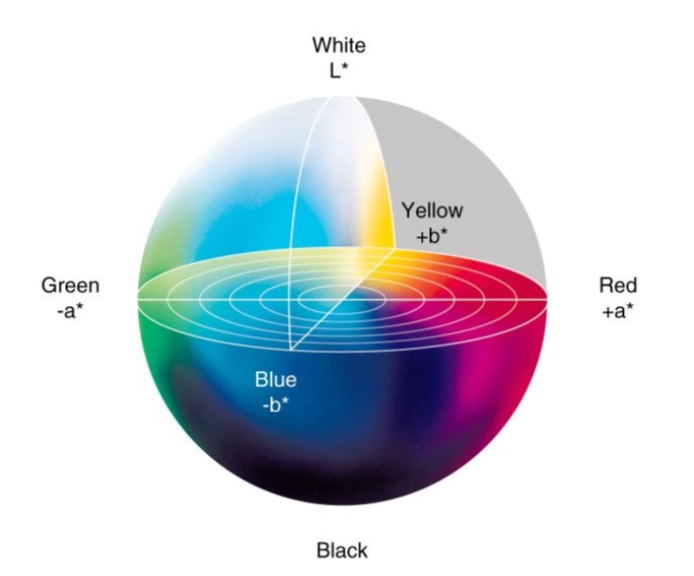
\includegraphics[width=170pt]{img/cielab.jpg}
  \caption{CIE Lab Color Space}
  \label{fig:cielab}
\end{figure}

\begin{equation}\label{DeltaE}
	\Delta E_{ab}= \sqrt{(L_{2}-L_{1})^2+(a_{2}-a_{1})^2+(b_{2}-b_{1})^2}
\end{equation}	
\\ In particular, from the result above it is possible to infer as follow:
\begin{itemize}
	\item when $0<\Delta E_{ab}<1$ an observer does not notice the difference;
	\item when $1\leq\Delta E_{ab}<2$ only experienced observers can notice the difference;
	\item when $2\leq\Delta E_{ab}<3.5$ unexperienced observers also notice the difference;
	\item when $3.5\leq\Delta E_{ab}<5$ clear difference in color is noticed;
	\item when $\Delta E_{ab}>5$ an observer notices two different colors.
\end{itemize}
\section{Resolution of Part 1}
The following section explains the choices you make in implementing the first part of the project.

\subsection{Dataset Reduction} 
The dataset is made up of 1269 samples of colors named "master" provided as a spectrum vector at a wavelength of 380nm to 800nm, the wavelenght of visible light. From these masters, distorted copies will need to be generated and then calculate the difference between the original colors and the copies as required by the project. It is possible to see (figure \ref{fig:dataset}), through a visual analysis of the dataset, that many master colors are "similar to each other" so the first operation was to skim the dataset by reducing the number of master colors. This helps reduce the computational cost of operations at first. In the next step, you will use the entire dataset. The solution used to reduce the dataset is to use the formula \ref{DeltaE} and eliminate the colors that have a difference between them, in terms of Lab coordinates, less than 3. After the reduction the number of samples in the dataset are 259 and the final dataset is shown in figure \ref{fig:reducteddataset}.
\begin{figure}
  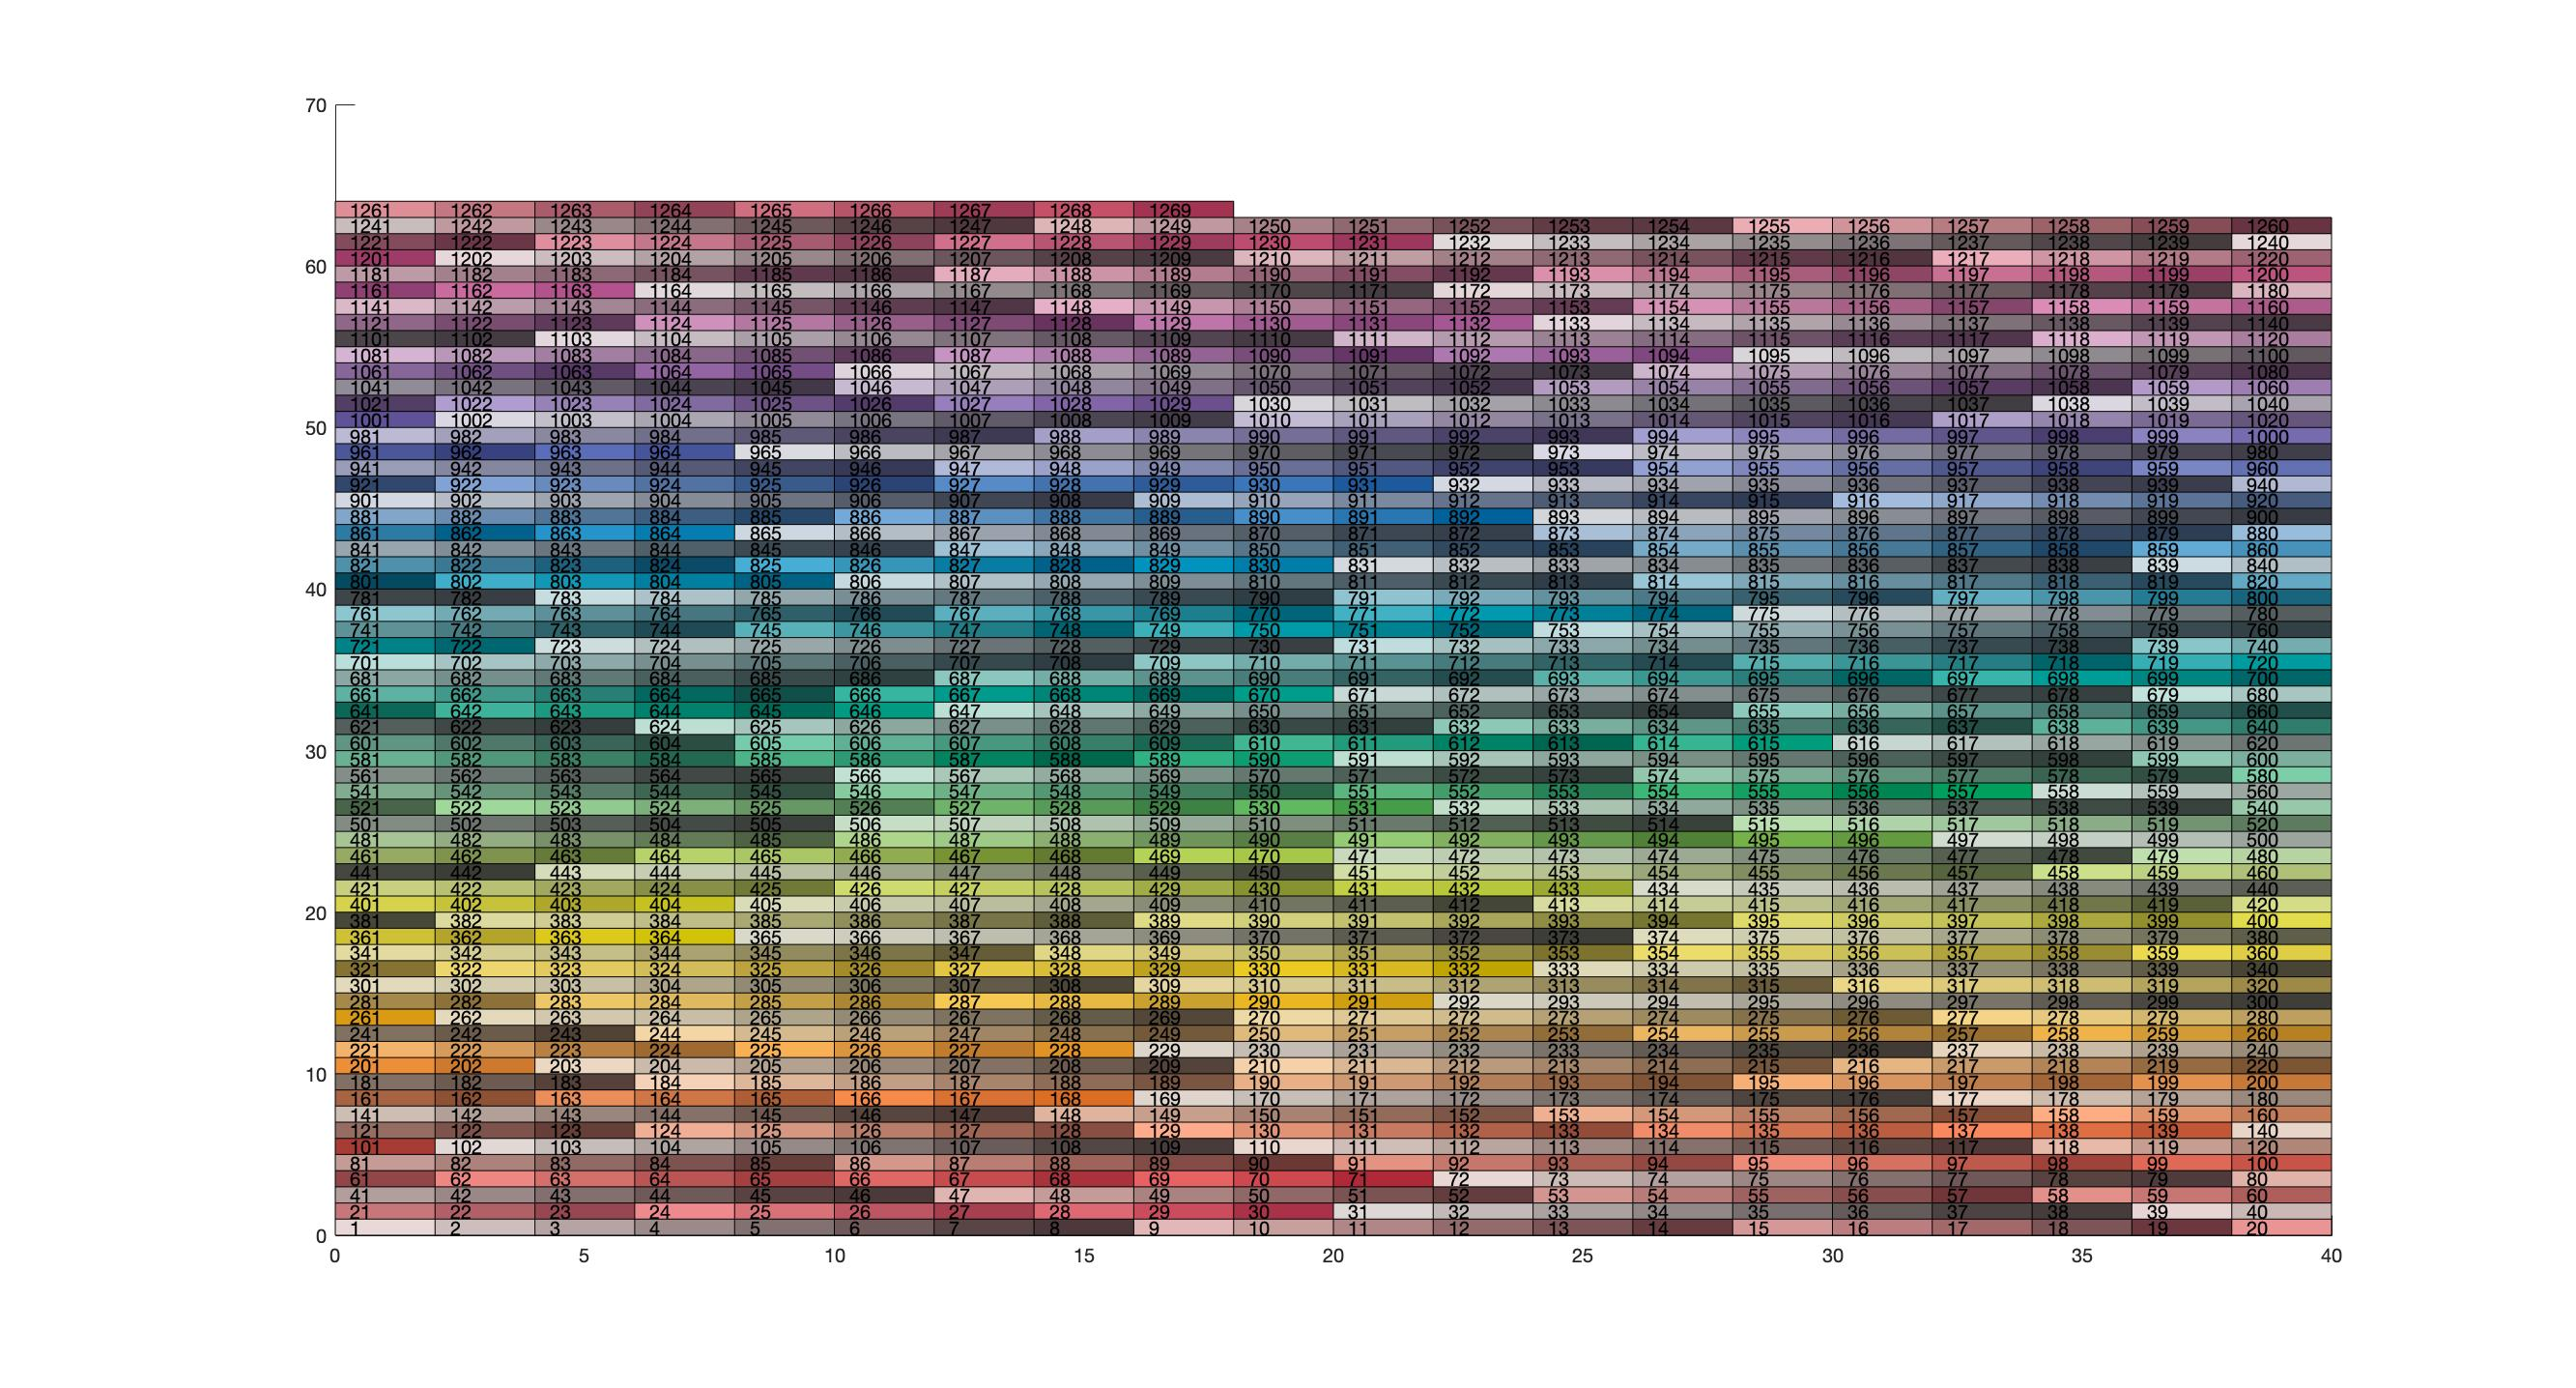
\includegraphics[width=\linewidth]{img/dataset.jpg}
  \caption{Original Dataset}
  \label{fig:dataset}
\end{figure}
\begin{figure}
  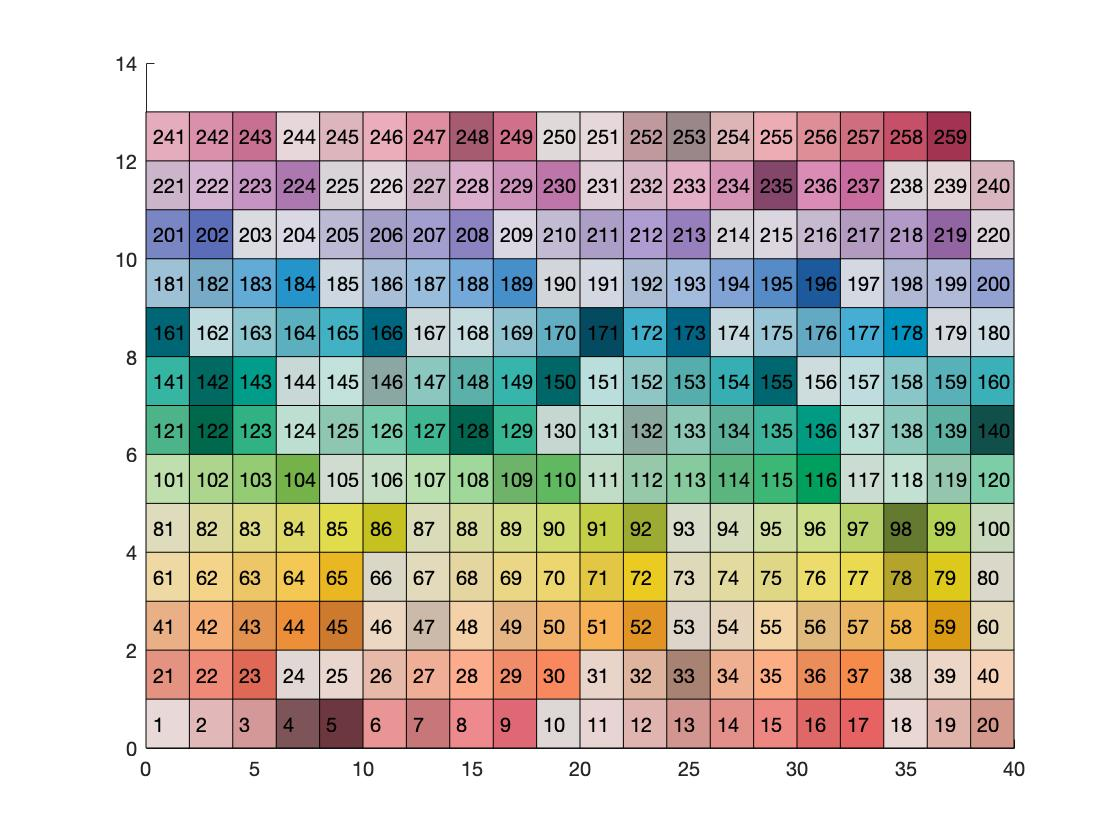
\includegraphics[width=\linewidth]{img/reducteddataset.jpg}
  \caption{Reduced Dataset}
  \label{fig:reducteddataset}
\end{figure}
\subsection{Copy Creation} 
The hypothesis used for the creation of the copies is the follow one: since the reference context is an industrial process, it is difficult to have a color difference greater than 5 i.e. a $\Delta E>5$. A script (noiseInterval.m) then evaluated the noise interval that could keep the percentage of copies low with $\Delta E>5$. Starting from an absent noise i.e. with a factor of 1, noise intervals were analyzed by increasing noise factor by 0.01. Table \ref{tab:tablepercentage} shows the results. The noise factor used is 1.14 and the range therefore varies randomly in [1,1.14]. To obtain a distortion of the spectrum, and then a copy, it is chosen to multiply the spectrum by a noise factor. An example can be shown in Figure \ref{fig:mastercopy} . The generation of copies was achieved by running the script \textbf{makeMasterCopyMatrix.m} that generated a number of 10 distorted copies for each master color in a noise range ranging from [1.00,1,14].
\begin{table}[h!]
  \begin{center}
    \label{tab:tablepercentage}
    \begin{tabular}{c|c|c|c|c|c} 
      \textbf{Interval} & \textbf{$0<\Delta E<1$} & \textbf{$1\leq\Delta E<2$}&\textbf{$2\leq\Delta E<3.5$}&\textbf{$3.5\leq\Delta E<5$}&\textbf{$\Delta E\geq5$}\\
       \hline
      $[1;1.12]$ & 0.25	 &0.29	&0.38	&0.07	& 0\\
      $[1;1.13]$ & 0.23 &	0.27 &	0.37 &	0.13 & 	0\\
      $[1;1.14]$ & 0.25 & 0.24 & 	0.33 &	0.18 &	0.001\\
      $[1;1.15]$ & 0.21 &	0.23 &	0.34 &	0.21 &	0.01\\
    \end{tabular}
    \caption{Percentage of Value in an interval of noise factors}
  \end{center}
\end{table}

\begin{figure}[h]
\center
  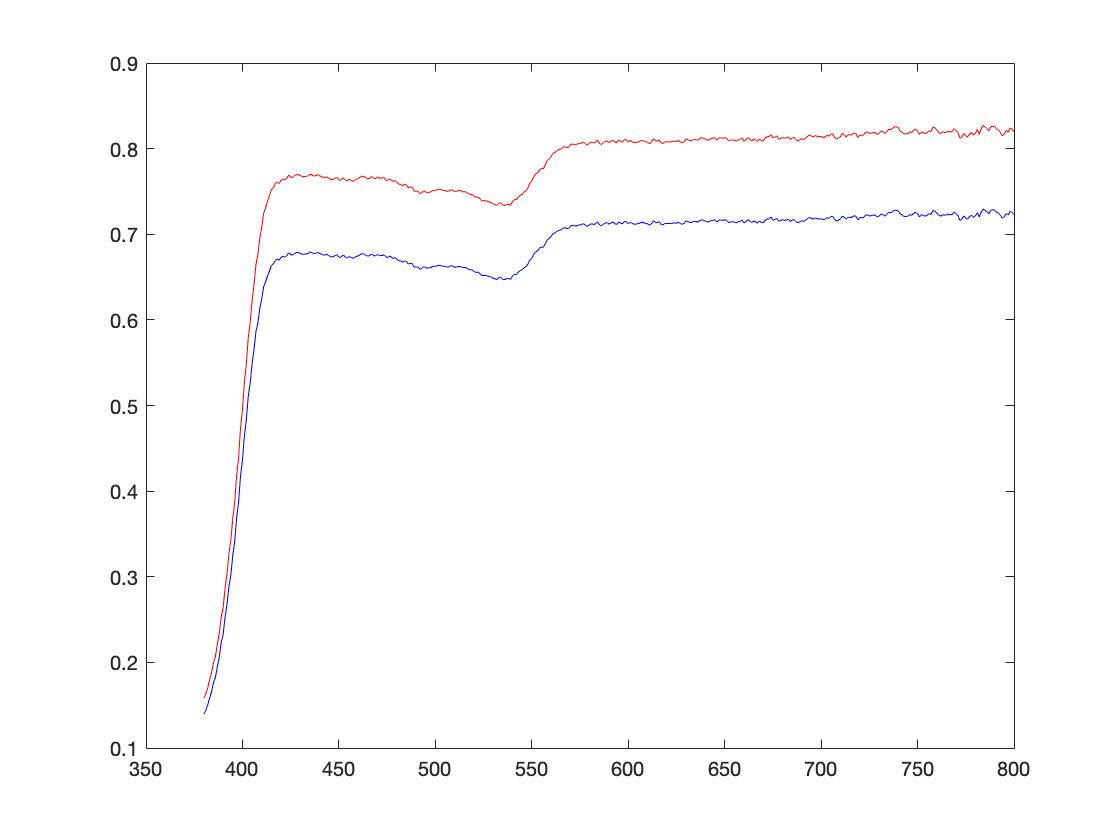
\includegraphics[width=300pt]{img/mastercopynoise.jpg}
  \caption{Master Color and Distorted Copy}
  \label{fig:mastercopy}
\end{figure}




\subsection{Feature Extraction} 
Before extracting spectra-related features, input reduction work was carried out for the neural network. The basic idea is to divide the spectra into intervals and calculate for each range the features to be proposed as input to the network. The characteristics of each range were chosen from the standard statistical features: \textbf{Mean, Median, Maximum, Minimum, Variance and Standard Deviation}.Since the mathematical \textbf{standard deviation} is the square root of the variance it was decided not to insert it in the characteristics since for the network it could be a redundant information (there is a very strong correlation about the two features). The choice of the number of intervals was made according to the following criterion: the spectrum is divided into intervals and the average is calculated for each interval. The new spectrum will have a number of values equal to the number of intervals. The new spectrum is interpolated (with a cubic interpolation) using the \textbf{interp1()} function of the Curve Fitting Toolbox and calculates how much interpolation differs from the original spectrum by the imse() function that calculates the mean squared error. If the value is very close to 0 then the interpolation represents a good approximation of the original function. In addition, the interval division also reduces the noise of the original spectra as shown in figure \ref{fig:interpolation} . After many experiments, the number of intervals chosen is 10 as the value of the average quadratic error settles into an order of magnitude ranging from 10\textsuperscript{-4} to 10\textsuperscript{-5}.
\begin{figure}[!h]
\center
  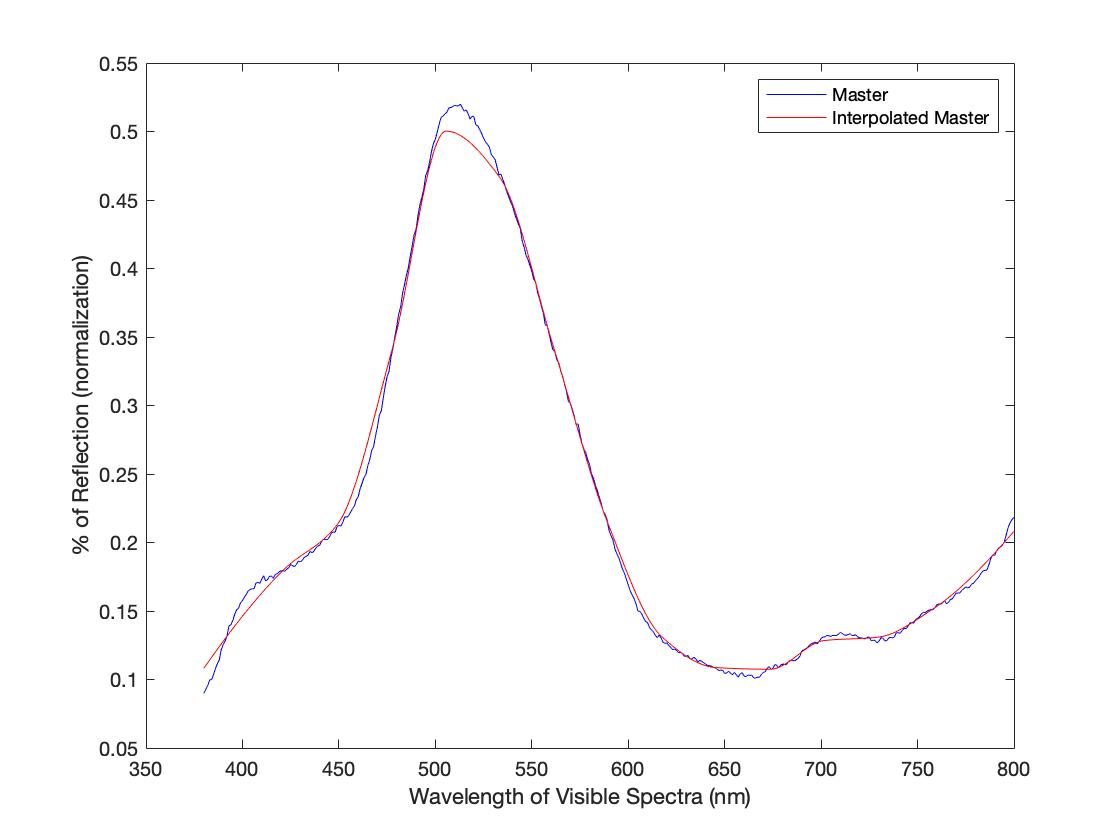
\includegraphics[width=300pt]{img/interpolation.jpg}
  \caption{Master Color and Interpolation}
  \label{fig:interpolation}
\end{figure}
For each interval it is possible to calculate the 6 statistic features above. In this way each interval will be characterized and described by its features. At the end of the process of extraction every spectra will be reducted from 421 values to 50 values so at the end, the number of input is reducted from 842 (421 for the master's spectra, 421 for the copy's spectra) to 100 (50 for the master's spectra, 50 for the copy's spectra) with an improvement of 88\% in terms of input numbers. Furthermore the number of inputs will be reduct in the phase of features selection. It is possible to see the main features of a spectra in figure \ref{fig:features}. 

\begin{figure}[!h]
\center
  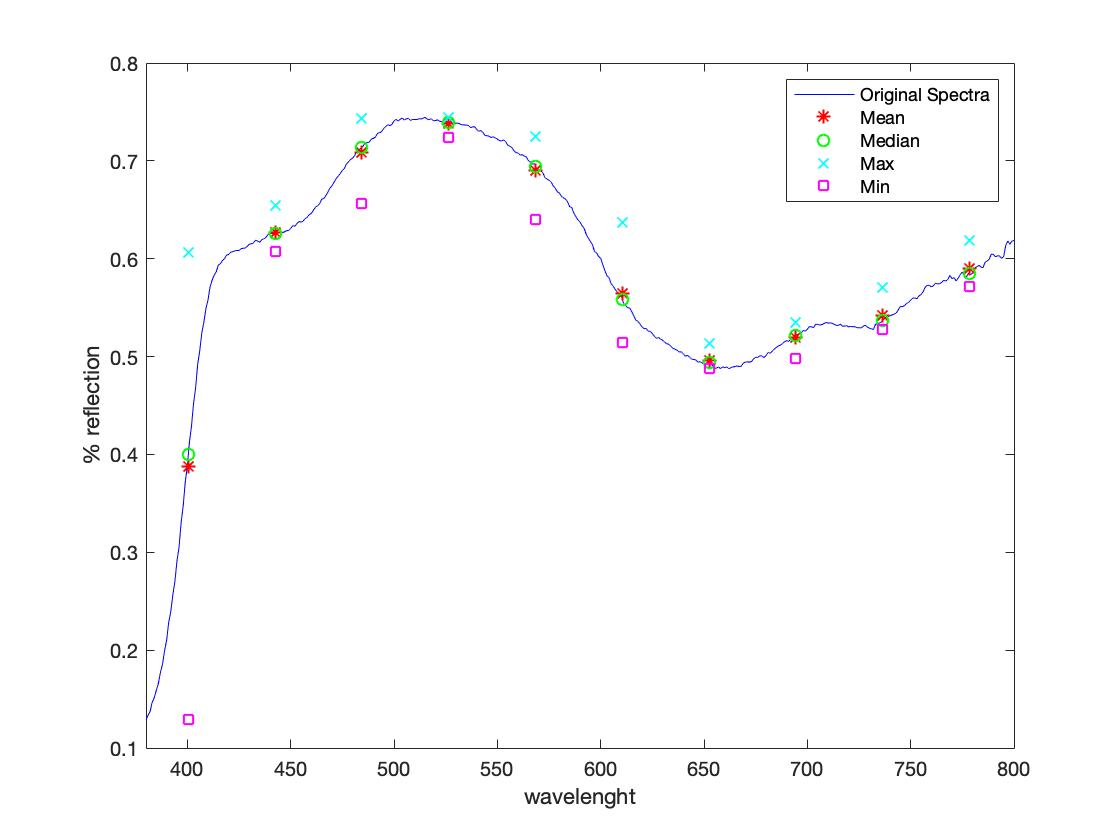
\includegraphics[width=300pt]{img/features.jpg}
  \caption{Features extracted from a spectra}
  \label{fig:features}
\end{figure}
 

\subsection{Feature Selection} 
After extracting the characteristics for each interval, it is possible to further decrease the number of inputs by selecting the characteristics. This selection was made through the selectionfs function. After numerous experiments, a correct tradeoff was chosen for the number of features extracted equal to 6. The stop criterion of the function was the performance of the neural network used for the selection of the characteristics and that is the mse. After many iterations and experiments the final columns included at the end are almost the same:  4 23 28 54 71 78. In this way the number of inputs are reducted from 100 to 6.
 
\subsection{Setting the Neural Network} 
The dataset is made up of 1269 samples of colors named "master" provided as a spectrum vector at a wavelength of 380nm to 800nm, the wavelenght of visible light. From these masters, distorted copies will need to be generated and then calculate the difference between the original colors and the copies as.
\end{document}



